\section{Bài toán}\label{sec:bai-toan}

Drone S500 của nhóm mang một bo camera riêng: ESP32-S3 N16R8 với cảm biến OV3660, gắn nhìn thẳng xuống đất. Bo phát luồng MJPEG qua Mobile Hotspot của laptop, mỗi khung là một JPEG 640$\times$480 nén ở mức chất lượng 12. Ngoài bãi bay, luồng đạt 2 đến 9 khung/s. Mọi xử lý AI chạy trên laptop (RTX 4060 Laptop 8 GB) trong phần mềm điều khiển IOT-CV, vì bo ESP32-S3 chỉ đủ sức nén và gửi ảnh.

Từ cùng một khung gốc, đồ án phải cho ra hai thứ. Thứ nhất là nhận diện: hộp $[x_1,y_1,x_2,y_2]$ kèm độ tin cậy cho lớp người, để web cảnh báo người vận hành. Thứ hai là ảnh rõ: một khung cùng cỡ, dễ nhìn hơn cho người ngồi trước màn hình. Hai đầu ra tách nhau: nhận diện chạy trên khung gốc, ảnh rõ chỉ phục vụ mắt người (Hình~\ref{fig:pipeline}). Luật đặt từ đầu là điểm số chỉ chấm trên khung bay thật; ảnh tự sinh được dùng để huấn luyện, không dùng để kết luận. Bài toán dùng kiến thức nâng cao chất lượng ảnh, hệ màu, nén JPEG và nhận dạng của học phần~\cite{baigiang,gonzalez}.

\begin{figure}[!htbp]
\centering
\resizebox{\textwidth}{!}{% Đường đi của một khung trong IOT-CV với ba gói ONNX (results/.../iotcv/README.md §1, bảng t9)
\begin{tikzpicture}[
  font=\scriptsize, node distance=3.5mm and 4.5mm,
  khoi/.style={draw=#1, fill=#1!12, rounded corners=2pt, line width=0.8pt, align=center, minimum height=11mm, text width=19mm},
  mui/.style={-{Stealth[length=2.2mm]}, line width=0.9pt, cXam},
]
\node[khoi=cHong] (cam) {\textbf{Camera}\\ESP32-S3 N16R8\\+ OV3660\\JPEG 640$\times$480};
\node[khoi=cVang, right=of cam, text width=17mm] (wifi) {\textbf{Wi-Fi}\\MJPEG qua HTTP\\2 đến 9 khung/s};
\node[khoi=cXanh, right=of wifi, text width=19mm] (gcs) {\textbf{Laptop}\\ONNX Runtime\\CUDA, RTX 4060\\Laptop 8 GB};
\node[khoi=cCam, above right=2mm and 7mm of gcs.east, anchor=south west, text width=23mm] (det) {\textbf{Tầng 1}\\detector YOLO11s\\gói ONNX nhận diện};
\node[khoi=cTim, right=of det, text width=19mm] (ver) {\textbf{Tầng 2}\\verifier EffNet-B0\\cắt 96 px, $s\geq0{,}35$};
\node[khoi=cLuc, right=of ver, text width=15mm] (trk) {\textbf{Tầng 3}\\track IoU 0,3\\$k=n=1$};
\node[khoi=cXanh, below right=2mm and 7mm of gcs.east, anchor=north west, text width=46mm] (enh) {\textbf{Ảnh rõ trực tiếp}: gói ONNX làm rõ\\bộ lọc cổ điển, bật sẵn};
\node[draw=cXam, rounded corners=2pt, fill=cXam!8, align=center, text width=15mm, minimum height=11mm, right=5mm of enh] (web) {\textbf{Web}\\luồng ``Ảnh rõ''};
\node[draw=cXam, rounded corners=2pt, fill=cXam!8, align=center, text width=15mm, minimum height=11mm, above=2mm of trk] (canh) {\textbf{Web}\\cảnh báo người};
\draw[mui] (cam) -- (wifi);
\draw[mui] (wifi) -- (gcs);
\draw[mui] (gcs.east) -- ++(3mm,0) |- (det.west);
\draw[mui] (gcs.east) -- ++(3mm,0) |- (enh.west);
\draw[mui] (det) -- (ver);
\draw[mui] (ver) -- (trk);
\draw[mui] (trk) -- (canh);
\draw[mui] (enh) -- (web);
\end{tikzpicture}
}
\caption[Đường đi của một khung trong IOT-CV]{Đường đi của một khung trong IOT-CV. Ba tầng nhận diện chạy trên khung gốc; ``Ảnh rõ'' là nhánh riêng cho người xem và bật sẵn.}
\label{fig:pipeline}
\end{figure}

Nhóm đo lỗi của camera trên 1\,115 khung dev của chuyến bay ngày 02/11/2026 (bản ghi \texttt{20261102-100941}); khung test không tham gia phép đo. Bảng~\ref{tab:camera} liệt kê các lỗi chính, Hình~\ref{fig:loi-camera} cho thấy chúng trên khung thật. Lỗi nặng nhất là ám hồng: ISP nhân hệ số cân bằng trắng cho R và B lớn hơn G, nên ở vùng gần bão hoà kênh G dừng trước, đường bê tông và mái tôn sáng thành mảng hồng. Hồ sơ đo này là đầu vào của bộ làm xấu D2 và của bộ lọc cổ điển.

\begin{table}[!htbp]
\centering\footnotesize
\caption[Lỗi ảnh đo trên 1\,115 khung dev]{Lỗi ảnh đo trên 1\,115 khung dev (hồ sơ \texttt{ov3660-esp32s3-q12-20261102}, bản 1.2.0). Số là trung vị, ngoặc là p5 và p95.}
\label{tab:camera}
\begin{tabularx}{\textwidth}{@{}l X l@{}}
\toprule
Lỗi & Đại lượng đo & Giá trị \\
\midrule
Ám hồng vùng sáng & tỉ lệ điểm có $R-G>25$ và $B-G>25$; khung có $>0{,}5\,\%$ điểm hồng & 0,17\,\% (0; 3,3\,\%); 31\,\% số khung \\
Mù như sương & dark channel ô 15 px (thang 0 đến 255) & 143,7 (134,6; 152,1) \\
Vỡ khối JPEG & tỉ số biên khối $8\times8$; bảng DQT & 2,68 (2,15; 3,52); Annex K $\times$ 0,75, 4:2:2 \\
Tối góc & tỉ số sáng góc/tâm; tiêu cự khớp $\cos^4$ & 0,81 (0,62; 0,93); 1\,016 px \\
Dải tối mép trái & bề rộng dải & 14 px (13; 16) \\
Nhoè & $\sigma$ PSF Gauss khớp từ MTF50 & 0,76 px \\
\bottomrule
\end{tabularx}
\end{table}

\begin{figure}[!htbp]
\centering
\begin{subfigure}[b]{0.43\textwidth}\centering
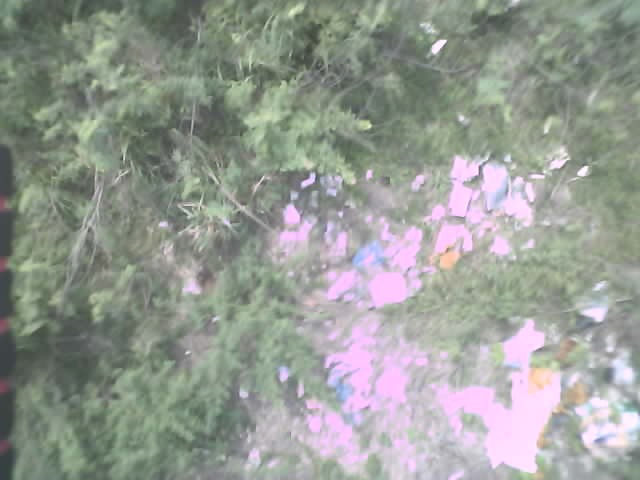
\includegraphics[width=\linewidth]{fig/art_full.jpg}
\caption{Khung \texttt{004\_01252}: mảng hồng, mù, tối góc}\end{subfigure}\hfill
\begin{subfigure}[b]{0.30\textwidth}\centering

\includegraphics[width=\linewidth]{fig/art_pink.jpg}
\caption{Mảng hồng phóng 4$\times$, thấy khối 8$\times$8}\end{subfigure}\hfill
\begin{subfigure}[b]{0.105\textwidth}\centering
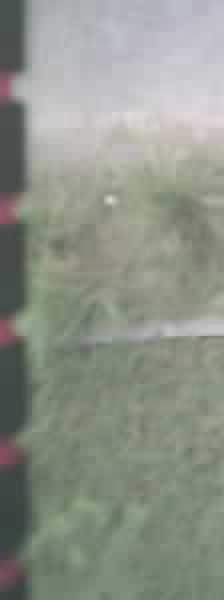
\includegraphics[width=\linewidth]{fig/art_strip.jpg}
\caption{Dải mép}\end{subfigure}\hfill
\begin{subfigure}[b]{0.13\textwidth}\centering

\includegraphics[width=\linewidth]{fig/art_block.jpg}
\caption{Biên khối, 8$\times$}\end{subfigure}
\caption[Lỗi của camera trên khung bay thật ngày 02/11/2026]{Lỗi của camera trên khung bay thật ngày 02/11/2026. Dải mép (c) rộng khoảng 14 cột nên mọi model bỏ 16 cột đầu.}
\label{fig:loi-camera}
\end{figure}

Một detector YOLO11s đứng một mình báo nhầm 0,881 hộp trên mỗi khung bay không người: túi rác, mảnh nhựa hồng, bóng người bị nhận thành người. Hệ của nhóm giải quyết hai chỗ: lọc báo nhầm bằng hai tầng đặt sau detector, và làm rõ ảnh bằng bộ lọc cổ điển chạy dưới dạng ONNX. Tập test 198 khung chỉ được chấm một lần, luật chọn ghi trước khi chạy.
